\documentclass[12pt]{article}
\usepackage{geometry}
\geometry{a4paper, margin=1in}
\usepackage{setspace}
\usepackage{graphicx}
\usepackage{amsmath, amssymb}
\usepackage{booktabs}
\usepackage{hyperref}
\usepackage{xcolor}

\setstretch{1}

\title{{A Model-Based Statistical Investigation of Factors Influencing Vehicle Fuel Efficiency}}
% \large Effects of Cylinders, Horsepower, Weight, and Model Year on Fuel Efficiency:\\ A $2^4$ Factorial Design Using Car Dataset}
\author{
Group members:
Feng Gu (T00751197),
Jiahui Yan (T00752485), \\
Emmanuella Onyejiaka (T00748938), 
Yuzhuo Ye (T00751492), \\
Taiwo Ogunkeye (T00751495)
}
\date{}

\begin{document}
\maketitle

\section{Introduction and Research Question}

Fuel efficiency remains one of the most important performance indicators in the automotive industry,
influencing both environmental impact and consumer cost. Previous studies \cite{ahmad2020, greene2017}
have shown {that some mechanical factors}, like engine size and horsepower can affect fuel consumption.

With the right combination of these factors, improvement on fuel efficiency has been proven achievable,
which promises the potential for developing more fuel-efficient vehicles by exploring optimal 
configurations on these factors and their interactions.
Motivated by this background, this project aims to examine how a series of car factors (controllable factors) affect the fuel efficiency (target variable).

\section{{Research Objectives}}

This project aims to systematically investigate the factors influencing automotive fuel efficiency through
statistically controls for major confounding factors. The primary objective is to examine how key automotive characteristics individually
and collectively affect miles per gallon (MPG) performance. Specifically, we seek to:
\begin{enumerate}
    \item Determine the main effects of each factor on fuel efficiency
    \item Identify potential interaction effects among these factors to understand how combinations of characteristics influence fuel performance
    \item Apply appropriate statistical analysis including assumption testing and effect size estimation
\end{enumerate}


\section{{Data Description}}
The data are from the Auto MPG Dataset
\footnote{Data source: \url{https://www.kaggle.com/datasets/uciml/autompg-dataset}}
from UCI Machine Learning Repository \cite{uciml2021autompg}, it contains 398 automobiles manufactured between 1970-1982.

The dataset includes nine variables: the dependent variable \textbf{mpg} and eight predictors including cylinders, displacement, horsepower, weight, 
acceleration, model year, origin, and car name,
\footnote{Here the car name is a long string with brand and model information.}
the variable meanings are provided in \textcolor{blue}{Table \ref{tab:dataset_summary}} and 
their distributions are shown in \textcolor{blue}{Figure \ref{fig:numerical_distributions_with_outliers}} in the Appendix.

\begin{table}[!h]
\centering
\caption{Summary of Variables in the Auto MPG Dataset}
\label{tab:dataset_summary}
\begin{tabular}{p{3cm}p{7cm}p{3cm}}
\toprule
\textbf{Variable} & \textbf{Description} & \textbf{Units / Type} \\
\midrule
mpg\(^*\)(target) & Miles per gallon (fuel efficiency) & $\text{miles}/\text{gallon}$ \\
cylinders & Number of engine cylinders & $\mathbb{N}$ \\
displacement & Engine displacement & $\text{in}^3$(cubic inches) \\
horsepower & Engine power output & $\text{hp}$ \\
weight & Vehicle weight & $\text{lb}$ \\
acceleration & Time to accelerate 0–60 mph & $\text{s}$ \\
model year & Year of manufacture (two-digit) & $\mathbb{N}$ \\
origin & Country/region of origin & $\{1,2,3\}$ \\
car name & Car make and model & $\text{string}$ \\
\bottomrule
\end{tabular}
\end{table}

The variable \textbf{car name} is a string and does not support distribution plots. We split its strings and extract the major car brands for 
all 398 samples, and the car brand distribution is shown in \textcolor{blue}{Figure \ref{fig:brand_distribution}} in the Appendix.

\section{Literature Review}

Contemporary automotive research employs statistical experimental design methodologies to investigate fuel efficiency factors. Jankovic and Magner \cite{jankovic2006fuel} used 
factorial design approaches including full-factorial and central composite designs to optimize automotive engine fuel economy. 
Najafi et al. \cite{najafi2015response} applied response surface methodology to investigate multiple engine parameters including f
uel blends and operating conditions to optimize both performance and emissions simultaneously. Win et al. \cite{win2005taguchi} 
implemented Taguchi methods to evaluate diesel engine operating parameters for minimizing noise, emissions, and fuel consumption.

Leveraging the findings and methods of previous studies in developing fuel-efficient vehicles,
Ahmad et al. \cite{ahmad2020} found 10\% weight reduction improves fuel economy by 8\%. 
Greene and Welch \cite{greene2017} showed higher cylinder counts reduce MPG due to increased energy requirements.
Li and Zhao \cite{li2022} observed newer models achieve better efficiency through improved engine management.



Compared to one-way effects, fewer studies examine comprehensive interaction effects between multiple mechanical, temporal, and geographical factors.
This project addresses this gap using factorial design and multiple regression analysis to quantify both individual and combined
influences on fuel efficiency.


\section{Overview of Experimental Design}


\subsection{Experimental Units and Design Considerations}

\textbf{Experimental Units:} This study employs an observational design using existing automotive data rather than a controlled experiment. 
Each of the 398 automobiles in the Auto MPG dataset represents an independent observational unit.


\textbf{Design Considerations:} While randomization is not applicable to this observational study, 
the dataset's comprehensive coverage across multiple manufacturers, model years, and geographic 
regions provides natural variation that supports robust statistical inference.
Potential confounding variables including transmission type, engine displacement, 
and manufacturing differences will be acknowledged as limitations. 
\subsection{Hypotheses and Statistical Models}

The following hypotheses will be tested to examine the relationships between automotive characteristics and fuel efficiency at $\alpha = 0.05$ significance level:


\subsubsection{ANOVA Model for Categorical Factors:}
\begin{align}
\text{MPG}_{ijk} &= \mu + \alpha_i + \beta_j + (\alpha\beta)_{ij} + \epsilon_{ijk}
\end{align}

\noindent where $i$ represents cylinder groups, $j$ represents origin groups, and $(\alpha\beta)_{ij}$ represents interaction effects.
The error term is tentatively assumed to follow \(\epsilon_{ijk} \sim N(0,\sigma^2)\) for observations within each group.

\begin{table}[h]
\centering
\caption{Main Effect Hypotheses for Automotive Fuel Efficiency Analysis}
\label{tab:main_hypotheses}
\begin{tabular}{p{2.5cm}p{6cm}p{6cm}}
\toprule
\textbf{Variable} & \textbf{Null Hypothesis ($H_0$)} & \textbf{Alternative Hypothesis ($H_1$)} \\
\midrule
Cylinders & Number of cylinders has no significant effect on MPG & Number of cylinders has a significant effect on MPG \\
\midrule
Origin & Country/region of origin has no significant effect on MPG & Country/region of origin has a significant effect on MPG \\
\midrule
Cylinders × Origin & There is no significant interaction effect between cylinders and origin on MPG & There is a significant interaction effect between cylinders and origin on MPG \\
\bottomrule
\end{tabular}
\end{table}

\subsubsection{Multiple Linear Regression Model for Continuous Factors:}

\begin{align}
\text{MPG} &= \beta_0 + \beta_1(\text{Cylinders}) + \beta_2(\text{Displacement}) + \beta_3(\text{Horsepower}) \nonumber \\
&\quad + \beta_4(\text{Weight}) + \beta_5(\text{Acceleration}) + \beta_6(\text{Model Year}) \nonumber \\
&\quad + \beta_7(\text{Origin}_2) + \beta_8(\text{Origin}_3) + \epsilon
\end{align}

\noindent where $\epsilon \sim N(0,\sigma^2)$ and Origin is dummy-coded with USA as reference category.

\begin{table}[!h]
\centering
\caption{Specific Directional Hypotheses}
\label{tab:directional_hypotheses}
\begin{tabular}{p{3cm}p{4.5cm}p{7cm}}
\toprule
\textbf{Relationship} & \textbf{Null Hypothesis($H_0$)} & \textbf{Alternative Hypothesis($H_1$)} \\
\midrule
Cylinders-MPG & $\beta_{\text{cylinders}} = 0$ & $\beta_{\text{cylinders}} < 0$ \newline (More cylinders decrease MPG) \\
\midrule
Weight-MPG & $\beta_{\text{weight}} = 0$ & $\beta_{\text{weight}} < 0$ \newline (Higher weight decreases MPG) \\
\midrule
Horsepower-MPG & $\beta_{\text{horsepower}} = 0$ & $\beta_{\text{horsepower}} < 0$ \newline (Higher horsepower decreases MPG) \\
\midrule
Model Year-MPG & $\beta_{\text{year}} = 0$ & $\beta_{\text{year}} > 0$ \newline (Newer cars have higher MPG) \\
\midrule
Origin Effect & $\mu_{\text{USA}} = \mu_{\text{Europe}} = \mu_{\text{Japan}}$ & At least one origin mean differs significantly \\
\bottomrule
\end{tabular}
\end{table}



\section{{Preliminary Analysis: One-Way ANOVA on Car Origin and Fuel Efficiency}}

% \subsection{One-Way ANOVA: Effect of Car Origin on Fuel Efficiency}

As a preliminary investigation, we conducted a one-way ANOVA to examine whether car origin (USA, Europe, Japan) 
significantly affects fuel efficiency, and this analysis serves as a foundational step to more complex multi-factor designs.

\textbf{Experimental Design:} The one-way ANOVA employed a completely randomized design with car origin 
as the single factor at three levels: Origin 1 (USA, n=249), Origin 2 (Europe, n=70), and Origin 3 (Japan, n=79). 
Each car represents an independent experimental unit, with MPG as the continuous response variable.

\textbf{Hypotheses Tested:}
\begin{itemize}
    \item $H_0$: $\mu_{\text{USA}} = \mu_{\text{Europe}} = \mu_{\text{Japan}}$ (all origin groups have equal mean MPG)
    \item $H_1$: At least one origin group has a significantly different mean MPG
\end{itemize}


\begin{figure}[!h]
    \centering
    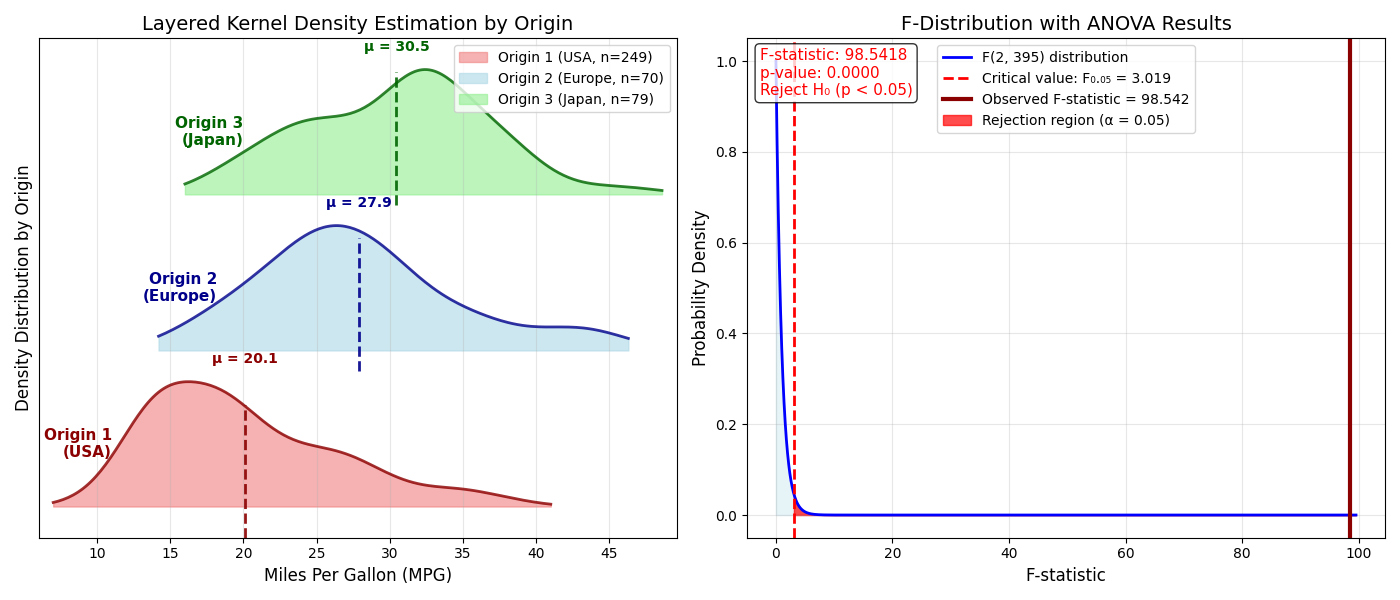
\includegraphics[width=0.9\textwidth]{../results/anova_origin_mpg.png}
    \caption{Preliminary ANOVA Results: Effect of Car Origin on Fuel Efficiency (MPG)}
    \label{fig:preliminary_anova}
\end{figure}



\begin{table}[h!]
\centering
\caption{One-Way ANOVA Results: Effect of Car Origin on Fuel Efficiency (MPG)}
\label{tab:anova_results}
\begin{tabular}{lc}
\toprule
\textbf{ANOVA Summary} & \textbf{Value} \\
\midrule
Null Hypothesis ($H_0$) & All group mpg means are equal \\
Alternative Hypothesis ($H_1$) & At least one group mpg mean differs \\
Significance level ($\alpha$) & 0.050 \\
\midrule
Total sample size ($N$) & 398 \\
Number of groups ($k$) & 3 \\
Degrees of freedom (Between groups) & 2 \\
Degrees of freedom (Within groups) & 395 \\
Critical $F$-value & 3.0186 \\
Observed $F$-statistic & 98.5418 \\
$p$-value & $< 0.001$ \\
\midrule
Statistical Decision & \textbf{Reject $H_0$} \\
Effect Size ($\eta^2$) & 0.3329 \\
\bottomrule
\end{tabular}
\end{table}

The ANOVA revealed a highly significant effect of car origin on fuel efficiency
\((F_{(2,395)} = 98.54\), \(p < 0.001\), $\eta^2$ = 0.333). Japanese cars showed highest efficiency (M = 30.45), 
followed by European (M = 27.89) and American cars (M = 20.08), leading to rejection of the null hypothesis.

This preliminary analysis confirms significant regional differences in automotive fuel efficiency, supporting 
the inclusion of origin as a key factor in subsequent multi-factorial designs.



\section{References}
\begin{thebibliography}{9}

\bibitem{ahmad2020}
Ahmad, N., et al. (2020). \textit{Weight reduction and fuel efficiency in automotive design: An integrated assessment}. Transportation Research Part D: Transport and Environment, 86, 102446.

\bibitem{greene2017}
Greene, D. L., \& Welch, T. (2017). \textit{Impact of engine size and vehicle weight on fuel economy: Policy implications}. Energy Policy, 108, 273–282.

\bibitem{li2022}
Li, F., \& Zhao, J. (2022). \textit{Advances in automotive efficiency: The role of model year innovation}. Applied Energy, 325, 119823.

\bibitem{uciml2021autompg}
U.S. Department of Energy. (2021). \textit{Auto MPG Dataset}. 
UCI Machine Learning Repository. Retrieved from \url{https://www.kaggle.com/datasets/uciml/autompg-dataset}

\bibitem{montgomery2019design}
Montgomery, D. C. (2019). \textit{Design and Analysis of Experiments} (9th ed.). John Wiley \& Sons.

\bibitem{jankovic2006fuel}
Jankovic, M., \& Magner, S. (2006). Fuel economy optimization in automotive engines. \textit{2006 American Control Conference}. IEEE. pp. 3334-3340.

\bibitem{najafi2015response}
Najafi, G., Ghobadian, B., Yusaf, T., Ardebili, S. M. S., \& Mamat, R. (2015).
Optimization of performance and exhaust emission parameters of a SI (spark ignition) engine with gasoline–ethanol
blended fuels using response surface methodology. \textit{Energy}, 90, 1815-1829.

\bibitem{win2005taguchi}
Win, Z., Gakkhar, R. P., Jain, S. C., \& Bhattacharya, M. (2005).
Investigation of diesel engine operating and injection system parameters for low noise, emissions,
and fuel consumption using Taguchi methods. \textit{Proceedings of the Institution of Mechanical Engineers,
Part D: Journal of Automobile Engineering}, 219(10), 1237-1251.

\end{thebibliography}

\clearpage
\section{Appendix}

% \subsection{Figures}
\begin{figure}[!h]
    \centering
    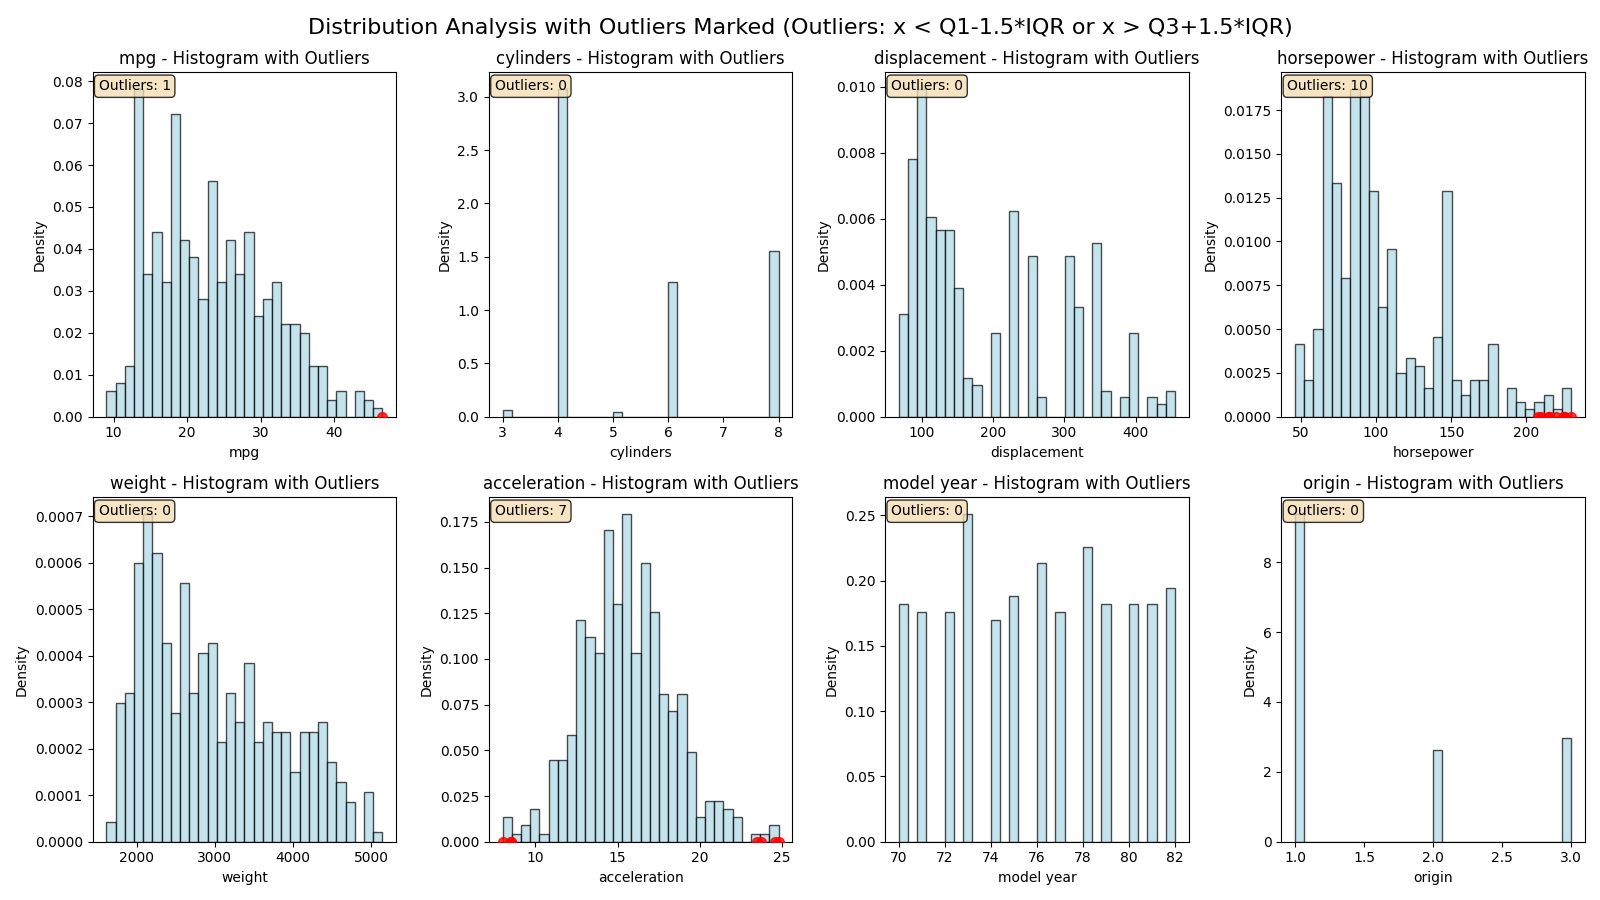
\includegraphics[width=0.8\textwidth]{../results/numerical_distributions_with_outliers.png}
    \caption{Distributions of Numerical Variables in the Auto MPG Dataset}
    \label{fig:numerical_distributions_with_outliers}
\end{figure}

\begin{figure}[!h]
    \centering
    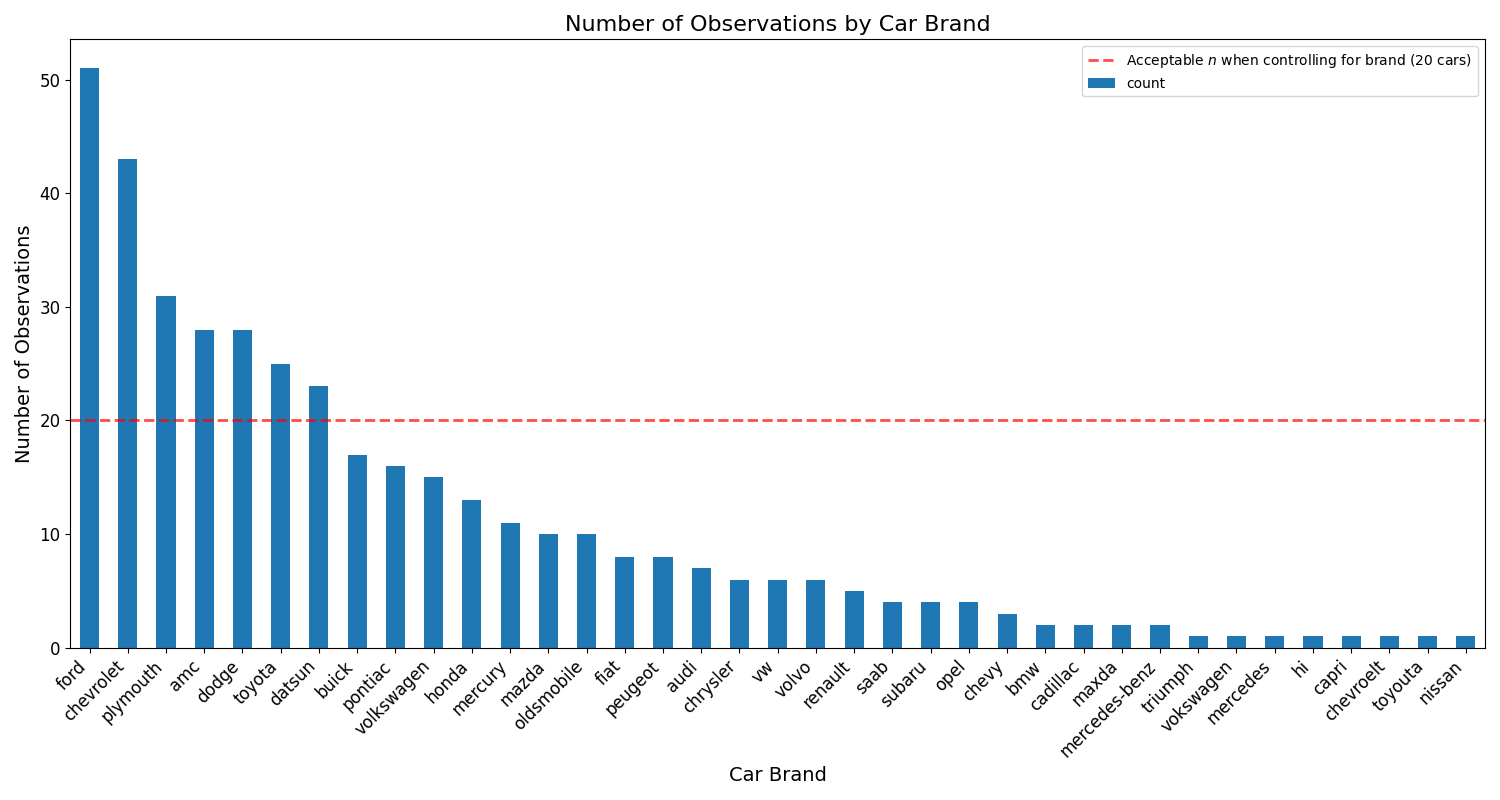
\includegraphics[width=0.8\textwidth]{../results/brand_distribution.png}
    \caption{Distribution of samples by Car Brand}
    \label{fig:brand_distribution}
\end{figure}

\begin{table}[!h]
\centering
\caption{Descriptive Statistics of Fuel Efficiency (MPG) by Car Origin}
\label{tab:descriptive_stats}
\begin{tabular}{lccc}
\toprule
\textbf{Origin} & \textbf{Sample Size ($n$)} & \textbf{Mean MPG} & \textbf{Standard Deviation} \\
\midrule
Origin 1 (USA) & 249 & 20.08 & 6.40 \\
Origin 2 (Europe) & 70 & 27.89 & 6.72 \\
Origin 3 (Japan) & 79 & 30.45 & 6.09 \\
\midrule
\textbf{Total} & \textbf{398} & \textbf{23.51} & \textbf{7.82} \\
\bottomrule
\end{tabular}
\end{table}

\subsection{Ethical Considerations}

Although the dataset is non-human and publicly available, ethical integrity is maintained by:

\begin{itemize}
    \item \textbf{Data Source:} \url{https://www.kaggle.com/datasets/uciml/autompg-dataset}
    \item \textbf{Privacy and Compliance:} Ensuring no personally identifiable information is used.
    \item \textbf{Fair Representation:} Avoiding selective reporting or p-hacking.
    \item \textbf{Academic Integrity:} Properly citing all sources and acknowledging dataset creators.
\end{itemize}




\end{document}
